\documentclass[11pt, a4paper]{book}
\renewcommand\familydefault{\sfdefault}

%%%%%%%%%%%%%%%%%%%%%%%%%%%%%%%%%%%%%%%%%
% The Legrand Orange Book
% Structural Definitions File
% Version 2.0 (9/2/15)
%
% Original author:
% Mathias Legrand (legrand.mathias@gmail.com) with modifications by:
% Vel (vel@latextemplates.com)
% 
% This file has been downloaded from:
% http://www.LaTeXTemplates.com
%
% License:
% CC BY-NC-SA 3.0 (http://creativecommons.org/licenses/by-nc-sa/3.0/)
%
%%%%%%%%%%%%%%%%%%%%%%%%%%%%%%%%%%%%%%%%%

%----------------------------------------------------------------------------------------
%	VARIOUS REQUIRED PACKAGES AND CONFIGURATIONS
%----------------------------------------------------------------------------------------

\usepackage[top=2.0cm,bottom=2.0cm,left=2.5cm,right=2cm,headsep=10pt,a4paper]{geometry} % Page margins

\usepackage{graphicx} % Required for including pictures
\graphicspath{{Pictures/}} % Specifies the directory where pictures are stored

\usepackage{lipsum} % Inserts dummy text

\usepackage{tikz} % Required for drawing custom shapes

\usepackage[english]{babel} % English language/hyphenation

\usepackage{enumitem} % Customize lists
\setlist{nolistsep} % Reduce spacing between bullet points and numbered lists

\usepackage{booktabs} % Required for nicer horizontal rules in tables

\usepackage{xcolor} % Required for specifying colors by name
% \definecolor{ocre}{RGB}{45,74,110} % Define the orange color used for highlighting throughout the book
\definecolor{ocre}{HTML}{3F729B}

%----------------------------------------------------------------------------------------
%	FONTS
%----------------------------------------------------------------------------------------

\usepackage{avant} % Use the Avantgarde font for headings
%\usepackage{times} % Use the Times font for headings
\usepackage{mathptmx} % Use the Adobe Times Roman as the default text font together with math symbols from the Sym­bol, Chancery and Com­puter Modern fonts

\usepackage{microtype} % Slightly tweak font spacing for aesthetics
\usepackage[utf8]{inputenc} % Required for including letters with accents
\usepackage[T1]{fontenc} % Use 8-bit encoding that has 256 glyphs

%----------------------------------------------------------------------------------------
%	BIBLIOGRAPHY AND INDEX
%----------------------------------------------------------------------------------------

\usepackage[style=alphabetic,citestyle=numeric,sorting=nyt,sortcites=true,autopunct=true,hyperref=true,abbreviate=false,backend=biber]{biblatex}
\addbibresource{bibliography.bib} % BibTeX bibliography file
\defbibheading{bibempty}{}

\usepackage{calc} % For simpler calculation - used for spacing the index letter headings correctly
\usepackage{makeidx} % Required to make an index
\makeindex % Tells LaTeX to create the files required for indexing

%----------------------------------------------------------------------------------------
%	MAIN TABLE OF CONTENTS
%----------------------------------------------------------------------------------------

\usepackage{titletoc} % Required for manipulating the table of contents

\contentsmargin{0cm} % Removes the default margin

% Part text styling
\titlecontents{part}[0cm]
{\addvspace{20pt}\centering\large\bfseries}
{}
{}
{}

% Chapter text styling
\titlecontents{chapter}[1.25cm] % Indentation
{\addvspace{12pt}\large\sffamily\bfseries} % Spacing and font options for chapters
{\color{ocre!60}\contentslabel[\Large\thecontentslabel]{1.25cm}\color{ocre}} % Chapter number
{\color{ocre}}  
{\color{ocre!60}\normalsize\;\titlerule*[.5pc]{.}\;\thecontentspage} % Page number

% Section text styling
\titlecontents{section}[1.25cm] % Indentation
{\addvspace{3pt}\sffamily\bfseries} % Spacing and font options for sections
{\contentslabel[\thecontentslabel]{1.25cm}} % Section number
{}
{\hfill\color{black}\thecontentspage} % Page number
[]

% Subsection text styling
\titlecontents{subsection}[1.25cm] % Indentation
{\addvspace{1pt}\sffamily\small} % Spacing and font options for subsections
{\contentslabel[\thecontentslabel]{1.25cm}} % Subsection number
{}
{\ \titlerule*[.5pc]{.}\;\thecontentspage} % Page number
[]

% List of figures
\titlecontents{figure}[0em]
{\addvspace{-5pt}\sffamily}
{\thecontentslabel\hspace*{1em}}
{}
{\ \titlerule*[.5pc]{.}\;\thecontentspage}
[]

% List of tables
\titlecontents{table}[0em]
{\addvspace{-5pt}\sffamily}
{\thecontentslabel\hspace*{1em}}
{}
{\ \titlerule*[.5pc]{.}\;\thecontentspage}
[]

%----------------------------------------------------------------------------------------
%	MINI TABLE OF CONTENTS IN PART HEADS
%----------------------------------------------------------------------------------------

% Chapter text styling
\titlecontents{lchapter}[0em] % Indenting
{\addvspace{15pt}\large\sffamily\bfseries} % Spacing and font options for chapters
{\color{ocre}\contentslabel[\Large\thecontentslabel]{1.25cm}\color{ocre}} % Chapter number
{}  
{\color{ocre}\normalsize\sffamily\bfseries\;\titlerule*[.5pc]{.}\;\thecontentspage} % Page number

% Section text styling
\titlecontents{lsection}[0em] % Indenting
{\sffamily\small} % Spacing and font options for sections
{\contentslabel[\thecontentslabel]{1.25cm}} % Section number
{}
{}

% Subsection text styling
\titlecontents{lsubsection}[.5em] % Indentation
{\normalfont\footnotesize\sffamily} % Font settings
{}
{}
{}

%----------------------------------------------------------------------------------------
%	PAGE HEADERS
%----------------------------------------------------------------------------------------

\usepackage{fancyhdr} % Required for header and footer configuration

\pagestyle{fancy}
\renewcommand{\chaptermark}[1]{\markboth{\sffamily\normalsize\bfseries\chaptername\ \thechapter.\ #1}{}} % Chapter text font settings
\renewcommand{\sectionmark}[1]{\markright{\sffamily\normalsize\thesection\hspace{5pt}#1}{}} % Section text font settings
\fancyhf{} \fancyhead[LE,RO]{\sffamily\normalsize\thepage} % Font setting for the page number in the header
\fancyhead[LO]{\rightmark} % Print the nearest section name on the left side of odd pages
\fancyhead[RE]{\leftmark} % Print the current chapter name on the right side of even pages
\renewcommand{\headrulewidth}{0.5pt} % Width of the rule under the header
\addtolength{\headheight}{2.5pt} % Increase the spacing around the header slightly
\renewcommand{\footrulewidth}{0pt} % Removes the rule in the footer
\fancypagestyle{plain}{\fancyhead{}\renewcommand{\headrulewidth}{0pt}} % Style for when a plain pagestyle is specified

% Removes the header from odd empty pages at the end of chapters
\makeatletter
\renewcommand{\cleardoublepage}{
\clearpage\ifodd\c@page\else
\hbox{}
\vspace*{\fill}
\thispagestyle{empty}
\newpage
\fi}

%----------------------------------------------------------------------------------------
%	THEOREM STYLES
%----------------------------------------------------------------------------------------

\usepackage{amsmath,amsfonts,amssymb,amsthm} % For math equations, theorems, symbols, etc

\newcommand{\intoo}[2]{\mathopen{]}#1\,;#2\mathclose{[}}
\newcommand{\ud}{\mathop{\mathrm{{}d}}\mathopen{}}
\newcommand{\intff}[2]{\mathopen{[}#1\,;#2\mathclose{]}}
\newtheorem{notation}{Notation}[chapter]

% Boxed/framed environments
\newtheoremstyle{ocrenumbox}% % Theorem style name
{0pt}% Space above
{0pt}% Space below
{\normalfont}% % Body font
{}% Indent amount
{\small\bf\sffamily\color{ocre}}% % Theorem head font
{\;}% Punctuation after theorem head
{0.25em}% Space after theorem head
{\small\sffamily\color{ocre}\thmname{#1}\nobreakspace\thmnumber{\@ifnotempty{#1}{}\@upn{#2}}% Theorem text (e.g. Theorem 2.1)
\thmnote{\nobreakspace\the\thm@notefont\sffamily\bfseries\color{black}---\nobreakspace#3.}} % Optional theorem note
\renewcommand{\qedsymbol}{$\blacksquare$}% Optional qed square

\newtheoremstyle{blacknumex}% Theorem style name
{5pt}% Space above
{5pt}% Space below
{\normalfont}% Body font
{} % Indent amount
{\small\bf\sffamily}% Theorem head font
{\;}% Punctuation after theorem head
{0.25em}% Space after theorem head
{\small\sffamily{\tiny\ensuremath{\blacksquare}}\nobreakspace\thmname{#1}\nobreakspace\thmnumber{\@ifnotempty{#1}{}\@upn{#2}}% Theorem text (e.g. Theorem 2.1)
\thmnote{\nobreakspace\the\thm@notefont\sffamily\bfseries---\nobreakspace#3.}}% Optional theorem note

\newtheoremstyle{blacknumbox} % Theorem style name
{0pt}% Space above
{0pt}% Space below
{\normalfont}% Body font
{}% Indent amount
{\small\bf\sffamily}% Theorem head font
{\;}% Punctuation after theorem head
{0.25em}% Space after theorem head
{\small\sffamily\thmname{#1}\nobreakspace\thmnumber{\@ifnotempty{#1}{}\@upn{#2}}% Theorem text (e.g. Theorem 2.1)
\thmnote{\nobreakspace\the\thm@notefont\sffamily\bfseries---\nobreakspace#3.}}% Optional theorem note

% Non-boxed/non-framed environments
\newtheoremstyle{ocrenum}% % Theorem style name
{5pt}% Space above
{5pt}% Space below
{\normalfont}% % Body font
{}% Indent amount
{\small\bf\sffamily\color{ocre}}% % Theorem head font
{\;}% Punctuation after theorem head
{0.25em}% Space after theorem head
{\small\sffamily\color{ocre}\thmname{#1}\nobreakspace\thmnumber{\@ifnotempty{#1}{}\@upn{#2}}% Theorem text (e.g. Theorem 2.1)
\thmnote{\nobreakspace\the\thm@notefont\sffamily\bfseries\color{black}---\nobreakspace#3.}} % Optional theorem note
\renewcommand{\qedsymbol}{$\blacksquare$}% Optional qed square
\makeatother

% Defines the theorem text style for each type of theorem to one of the three styles above
\newcounter{dummy} 
\numberwithin{dummy}{section}
\theoremstyle{ocrenumbox}
\newtheorem{theoremeT}[dummy]{Theorem}
\newtheorem{problem}{Problem}[chapter]
\newtheorem{exerciseT}{Exercise}[chapter]
\theoremstyle{blacknumex}
\newtheorem{exampleT}{Example}[chapter]
\theoremstyle{blacknumbox}
\newtheorem{vocabulary}{Vocabulary}[chapter]
\newtheorem{definitionT}{Definition}[section]
\newtheorem{corollaryT}[dummy]{Corollary}
\theoremstyle{ocrenum}
\newtheorem{proposition}[dummy]{Proposition}

%----------------------------------------------------------------------------------------
%	DEFINITION OF COLORED BOXES
%----------------------------------------------------------------------------------------

\RequirePackage[framemethod=default]{mdframed} % Required for creating the theorem, definition, exercise and corollary boxes

% Theorem box
\newmdenv[skipabove=7pt,
skipbelow=7pt,
backgroundcolor=black!5,
linecolor=ocre,
innerleftmargin=5pt,
innerrightmargin=5pt,
innertopmargin=5pt,
leftmargin=0cm,
rightmargin=0cm,
innerbottommargin=5pt]{tBox}

% Exercise box	  
\newmdenv[skipabove=7pt,
skipbelow=7pt,
rightline=false,
leftline=true,
topline=false,
bottomline=false,
backgroundcolor=ocre!10,
linecolor=ocre,
innerleftmargin=5pt,
innerrightmargin=5pt,
innertopmargin=5pt,
innerbottommargin=5pt,
leftmargin=0cm,
rightmargin=0cm,
linewidth=4pt]{eBox}	

% Definition box
\newmdenv[skipabove=7pt,
skipbelow=7pt,
rightline=false,
leftline=true,
topline=false,
bottomline=false,
linecolor=ocre,
innerleftmargin=5pt,
innerrightmargin=5pt,
innertopmargin=0pt,
leftmargin=0cm,
rightmargin=0cm,
linewidth=4pt,
innerbottommargin=0pt]{dBox}	

% Corollary box
\newmdenv[skipabove=7pt,
skipbelow=7pt,
rightline=false,
leftline=true,
topline=false,
bottomline=false,
linecolor=gray,
backgroundcolor=black!5,
innerleftmargin=5pt,
innerrightmargin=5pt,
innertopmargin=5pt,
leftmargin=0cm,
rightmargin=0cm,
linewidth=4pt,
innerbottommargin=5pt]{cBox}

% Creates an environment for each type of theorem and assigns it a theorem text style from the "Theorem Styles" section above and a colored box from above
\newenvironment{theorem}{\begin{tBox}\begin{theoremeT}}{\end{theoremeT}\end{tBox}}
\newenvironment{exercise}{\begin{eBox}\begin{exerciseT}}{\hfill{\color{ocre}\tiny\ensuremath{\blacksquare}}\end{exerciseT}\end{eBox}}				  
\newenvironment{definition}{\begin{dBox}\begin{definitionT}}{\end{definitionT}\end{dBox}}	
\newenvironment{example}{\begin{exampleT}}{\hfill{\tiny\ensuremath{\blacksquare}}\end{exampleT}}		
\newenvironment{corollary}{\begin{cBox}\begin{corollaryT}}{\end{corollaryT}\end{cBox}}	

%----------------------------------------------------------------------------------------
%	REMARK ENVIRONMENT
%----------------------------------------------------------------------------------------

\newenvironment{remark}{\par\vspace{10pt}\small % Vertical white space above the remark and smaller font size
\begin{list}{}{
\leftmargin=35pt % Indentation on the left
\rightmargin=25pt}\item\ignorespaces % Indentation on the right
\makebox[-2.5pt]{\begin{tikzpicture}[overlay]
\node[draw=ocre!60,line width=1pt,circle,fill=ocre!25,font=\sffamily\bfseries,inner sep=2pt,outer sep=0pt] at (-15pt,0pt){\textcolor{ocre}{R}};\end{tikzpicture}} % Orange R in a circle
\advance\baselineskip -1pt}{\end{list}\vskip5pt} % Tighter line spacing and white space after remark

%----------------------------------------------------------------------------------------
%	SECTION NUMBERING IN THE MARGIN
%----------------------------------------------------------------------------------------

\makeatletter
\renewcommand{\@seccntformat}[1]{\llap{\textcolor{ocre}{\csname the#1\endcsname}\hspace{1em}}}                    
\renewcommand{\section}{\@startsection{section}{1}{\z@}
{-4ex \@plus -1ex \@minus -.4ex}
{1ex \@plus.2ex }
{\normalfont\large\sffamily\bfseries}}
\renewcommand{\subsection}{\@startsection {subsection}{2}{\z@}
{-3ex \@plus -0.1ex \@minus -.4ex}
{0.5ex \@plus.2ex }
{\normalfont\sffamily\bfseries}}
\renewcommand{\subsubsection}{\@startsection {subsubsection}{3}{\z@}
{-2ex \@plus -0.1ex \@minus -.2ex}
{.2ex \@plus.2ex }
{\normalfont\small\sffamily\bfseries}}                        
\renewcommand\paragraph{\@startsection{paragraph}{4}{\z@}
{-2ex \@plus-.2ex \@minus .2ex}
{.1ex}
{\normalfont\small\sffamily\bfseries}}

%----------------------------------------------------------------------------------------
%	PART HEADINGS
%----------------------------------------------------------------------------------------

% numbered part in the table of contents
\newcommand{\@mypartnumtocformat}[2]{%
\setlength\fboxsep{0pt}%
\noindent\colorbox{ocre!20}{\strut\parbox[c][.7cm]{\ecart}{\color{ocre!70}\Large\sffamily\bfseries\centering#1}}\hskip\esp\colorbox{ocre!40}{\strut\parbox[c][.7cm]{\linewidth-\ecart-\esp}{\Large\sffamily\centering#2}}}%
%%%%%%%%%%%%%%%%%%%%%%%%%%%%%%%%%%
% unnumbered part in the table of contents
\newcommand{\@myparttocformat}[1]{%
\setlength\fboxsep{0pt}%
\noindent\colorbox{ocre!40}{\strut\parbox[c][.7cm]{\linewidth}{\Large\sffamily\centering#1}}}%
%%%%%%%%%%%%%%%%%%%%%%%%%%%%%%%%%%
\newlength\esp
\setlength\esp{4pt}
\newlength\ecart
\setlength\ecart{1.2cm-\esp}
\newcommand{\thepartimage}{}%
\newcommand{\partimage}[1]{\renewcommand{\thepartimage}{#1}}%
\def\@part[#1]#2{%
\ifnum \c@secnumdepth >-2\relax%
\refstepcounter{part}%
\addcontentsline{toc}{part}{\texorpdfstring{\protect\@mypartnumtocformat{\thepart}{#1}}{\partname~\thepart\ ---\ #1}}
\else%
\addcontentsline{toc}{part}{\texorpdfstring{\protect\@myparttocformat{#1}}{#1}}%
\fi%
\startcontents%
\markboth{}{}%
{\thispagestyle{empty}%
\begin{tikzpicture}[remember picture,overlay]%
\node at (current page.north west){\begin{tikzpicture}[remember picture,overlay]%	
\fill[ocre!20](0cm,0cm) rectangle (\paperwidth,-\paperheight);
\node[anchor=north] at (4cm,-3.25cm){\color{ocre!40}\fontsize{220}{100}\sffamily\bfseries\thepart}; 
\node[anchor=south east] at (\paperwidth-1cm,-\paperheight+1cm){\parbox[t][][t]{8.5cm}{
\printcontents{l}{0}{\setcounter{tocdepth}{1}}%
}};
\node[anchor=north east] at (\paperwidth-1.5cm,-3.25cm){\parbox[t][][t]{15cm}{\strut\raggedleft\color{white}\fontsize{30}{30}\sffamily\bfseries#2}};
\end{tikzpicture}};
\end{tikzpicture}}%
\@endpart}
\def\@spart#1{%
\startcontents%
\phantomsection
{\thispagestyle{empty}%
\begin{tikzpicture}[remember picture,overlay]%
\node at (current page.north west){\begin{tikzpicture}[remember picture,overlay]%	
\fill[ocre!20](0cm,0cm) rectangle (\paperwidth,-\paperheight);
\node[anchor=north east] at (\paperwidth-1.5cm,-3.25cm){\parbox[t][][t]{15cm}{\strut\raggedleft\color{white}\fontsize{30}{30}\sffamily\bfseries#1}};
\end{tikzpicture}};
\end{tikzpicture}}
\addcontentsline{toc}{part}{\texorpdfstring{%
\setlength\fboxsep{0pt}%
\noindent\protect\colorbox{ocre!40}{\strut\protect\parbox[c][.7cm]{\linewidth}{\Large\sffamily\protect\centering #1\quad\mbox{}}}}{#1}}%
\@endpart}
\def\@endpart{\vfil\newpage
\if@twoside
\if@openright
\null
\thispagestyle{empty}%
\newpage
\fi
\fi
\if@tempswa
\twocolumn
\fi}

%----------------------------------------------------------------------------------------
%	CHAPTER HEADINGS
%----------------------------------------------------------------------------------------

% A switch to conditionally include a picture, implemented by  Christian Hupfer
\newif\ifusechapterimage
\usechapterimagetrue
\newcommand{\thechapterimage}{}%
\newcommand{\chapterimage}[1]{\ifusechapterimage\renewcommand{\thechapterimage}{#1}\fi}%
\newcommand{\autodot}{.}
\def\@makechapterhead#1{%
{\parindent \z@ \raggedright \normalfont
\ifnum \c@secnumdepth >\m@ne
\if@mainmatter
\begin{tikzpicture}[remember picture,overlay]
\node at (current page.north west)
{\begin{tikzpicture}[remember picture,overlay]
\node[anchor=north west,inner sep=0pt] at (0,0) {\ifusechapterimage\includegraphics[width=\paperwidth]{\thechapterimage}\fi};
\draw[anchor=west] (\Gm@lmargin,-9cm) node [line width=2pt,rounded corners=15pt,draw=ocre,fill=white,fill opacity=0.5,inner sep=15pt]{\strut\makebox[22cm]{}};
\draw[anchor=west] (\Gm@lmargin+.3cm,-9cm) node {\huge\sffamily\bfseries\color{black}\thechapter\autodot~#1\strut};
\end{tikzpicture}};
\end{tikzpicture}
\else
\begin{tikzpicture}[remember picture,overlay]
\node at (current page.north west)
{\begin{tikzpicture}[remember picture,overlay]
\node[anchor=north west,inner sep=0pt] at (0,0) {\ifusechapterimage\includegraphics[width=\paperwidth]{\thechapterimage}\fi};
\draw[anchor=west] (\Gm@lmargin,-9cm) node [line width=2pt,rounded corners=15pt,draw=ocre,fill=white,fill opacity=0.5,inner sep=15pt]{\strut\makebox[22cm]{}};
\draw[anchor=west] (\Gm@lmargin+.3cm,-9cm) node {\huge\sffamily\bfseries\color{black}#1\strut};
\end{tikzpicture}};
\end{tikzpicture}
\fi\fi\par\vspace*{270\p@}}}

%-------------------------------------------
% PIETRO
%-------------------------------------------

\def\@makeschapterhead#1{%
\begin{tikzpicture}[remember picture,overlay]
\node at (current page.north west)
{\begin{tikzpicture}[remember picture,overlay]
\node[anchor=north west,inner sep=0pt] at (0,0) {\ifusechapterimage\includegraphics[width=\paperwidth]{\thechapterimage}\fi};
\draw[anchor=west] (\Gm@lmargin,-9cm) node [line width=2pt,rounded corners=15pt,draw=ocre,fill=white,fill opacity=0.5,inner sep=15pt]{\strut\makebox[22cm]{}};
\draw[anchor=west] (\Gm@lmargin+.3cm,-9cm) node {\huge\sffamily\bfseries\color{black}#1\strut};
\end{tikzpicture}};
\end{tikzpicture}
\par\vspace*{270\p@}}
\makeatother

%----------------------------------------------------------------------------------------
%	HYPERLINKS IN THE DOCUMENTS
%----------------------------------------------------------------------------------------

\usepackage{hyperref}
\hypersetup{hidelinks,colorlinks=false,breaklinks=true,urlcolor= ocre,bookmarksopen=false,pdftitle={Title},pdfauthor={Author}}
\usepackage{bookmark}
\bookmarksetup{
open,
numbered,
addtohook={%
\ifnum\bookmarkget{level}=0 % chapter
\bookmarksetup{bold}%
\fi
\ifnum\bookmarkget{level}=-1 % part
\bookmarksetup{color=ocre,bold}%
\fi
}
}
 % Insert the commands.tex file which contains the majority of the structure behind the template
\usepackage{multicol}
\usepackage{wrapfig}
\newcommand{\mail}[1]{\href{mailto:#1}{\texttt{#1}}}
\newcommand{\member}[2]{{\textbf{#1}\\}{#2}}
\newcommand{\myaut}[1]{{\underline{#1}}}


%\setlength{\columnseprule}{0.5pt}
%\newcommand{\mail}[1]{\href{mailto:#1}{\texttt{#1}}}
%\newcommand{\member}[2]{{\textbf{#1}\\}{#2}}
%\newcommand{\myaut}[1]{{\underline{#1}}}

\hyphenation{aspects}

\begin{document}

\begingroup
\thispagestyle{empty}
\begin{tikzpicture}[remember picture,overlay]
\coordinate [below=12cm] (midpoint) at (current page.north);
\node at (current page.north west)
{\begin{tikzpicture}[remember picture,overlay]
\node[anchor=north west,inner sep=0pt] at (0,0) {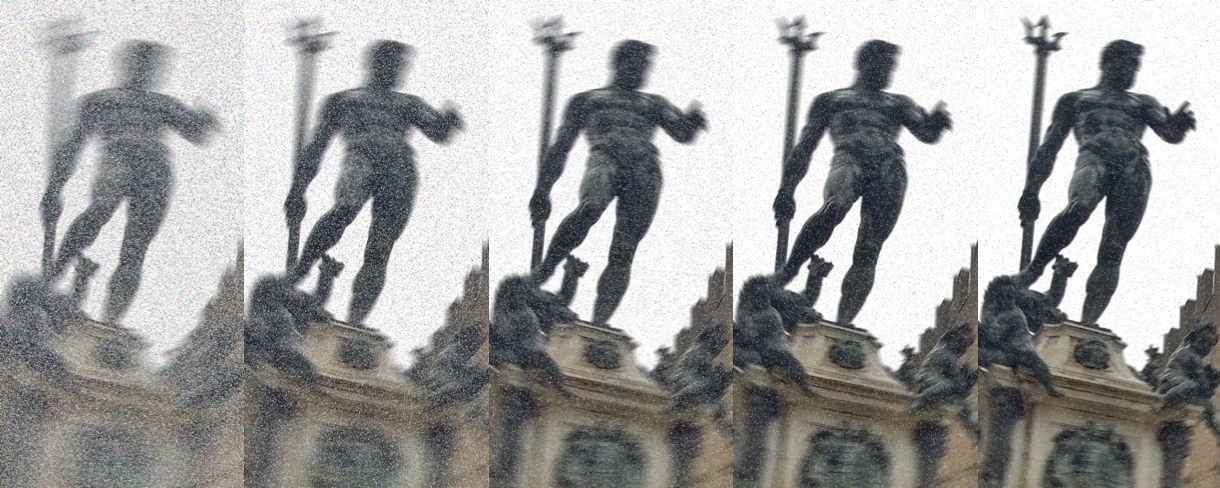
\includegraphics[width=\paperwidth]{images/nettuni.png}}; % Background
\draw[anchor=north] (midpoint) node [fill=myblue!30!white,fill opacity=0.6,text opacity=1,inner sep=1cm]{\Huge\centering\bfseries\sffamily\parbox[c][][t]{\paperwidth}{\centering SIAM Conference on IMAGING SCIENCE\\ Program and Abstracts\\[15pt] % Book title
{\Large June 5-8, 2018}\\[20pt] % Subtitle
{\huge University of Bologna, Italy}}}; % Author name
\end{tikzpicture}};
\end{tikzpicture}
\vfill
\endgroup
%\maketitle

%----------------------------------------------------------------------------------------
%	CONFERENCE THEMES
%----------------------------------------------------------------------------------------

\newpage
~\vfill
\thispagestyle{empty}

\noindent \textsc{https://siam-is18.dm.unibo.it}

\bigskip

\noindent This conference is the biennial activity of the SIAM Activity Group on Imaging Science.

\vspace{0.5cm}

\noindent The SIAM Activity Group on Imaging Science brings together SIAM members and other scientists and engineers with an interest 
in the mathematical and computational aspects of imaging.
The activity group organizes the biennial SIAM Conference on Imaging Science, awards the SIAG/IS Best Paper Prize
every two years to the authors of the best paper on mathematical and computational aspects of imaging, awards the SIAG/IS 
Early Career Prize to an outstanding early career researcher in the field of imaging science, and maintains a wiki, a
member directory, and an electronic mailing list.

\newpage

\section*{Conference Themes}

Reconstruction, enhancement, segmentation, analysis, registration, compression, representation, tomography, machine learning and tracking of two and three dimensional images are vital to many areas of science, medicine, and engineering. The increasingly sophisticated mathematical, statistical and computational methods employed in these research areas are referred to as \emph{Imaging Science}.\\ 
These techniques include transform and orthogonal series methods, nonlinear optimization, numerical linear algebra, integral equations, partial differential equations, Bayesian and other statistical inverse estimation methods, operator theory, differential geometry, information theory, interpolation and approximation, inverse problems, computer graphics and vision, stochastic processes, and others.

\smallskip

SIAM-IS18 will exchange research results and address open issues in all aspects of imaging science
and provide a forum for the presentation of work in imaging science.



\section*{Committee}

\bigskip
\noindent \textbf{\color{siamblue}General Co-Chairs}
\bigskip

\begin{itemize}
  \item[] \member{Omar Ghattas}{University of Texas at Austin, USA}
  \item[] \member{Fiorella Sgallari}{University of Bologna}
\end{itemize}

\bigskip
\noindent \textbf{\color{siamblue}Scientific Committee}
\bigskip

\begin{itemize}
  \item[] \member{Marcelo Bertalm\'io}{University Pompeu Fabra, Spain}
  \item[] \member{Julianne Chung}{Virginia Tech., USA}
  \item[] \member{Per Christian Hansen}{Technical University of Denmark, Denmark }
  \item[] \member{Jari Kaipio}{University of Auckland, New Zealand}
  \item[] \member{Eric Miller}{Tufts University, USA}
  \item[] \member{Mila Nikolova}{CNRS ENS Cachan, France}
  \item[] \member{Ronny Ramlau}{Kepler University Linz, Austria and Johann Radon Institute, Austria}
  \item[] \member{Carola Sch\"{o}nlieb}{University of Cambridge, United Kingdom}
  \item[] \member{Gabriele Steidl}{Tech.Univ. Kaiserslautern, Germany}
  \item[] \member{Xue-Cheng Tai}{Hong Kong Baptist University, China }
  \item[] \member{Laura Waller}{University of California Berkeley, USA }
  \item[] \member{Brendt Wohlberg}{Los Alamos National Laboratory, USA}
\end{itemize}

\bigskip
\noindent\textbf{\color{siamblue}Organizing Committee}
\bigskip

\begin{itemize}
  \item[] \member{Carolina Beccari}{Dept. Mathematics, University of Bologna}
  \item[] \member{Giulio Casciola}{Dept. Mathematics, University of Bologna}
  \item[] \member{Salvatore Cuomo}{Dept. Mathematics and Applications ``Renato Caccioppoli'', University of Naples}
  \item[] \member{Luigi Di Stefano}{Dept. Computer Science and Engineering, University of Bologna}
  \item[] \member{Giovanni Dore}{Dept. Mathematics, University of Bologna}
  \item[] \member{Maurizio Falcone}{Dept. Mathematics, University of Roma ``La Sapienza''}
  \item[] \member{Luca Formaggia}{Department of Mathematics, Politecnico di Milano}
  \item[] \member{Patrizio Frosini}{Dept. Mathematics, University of Bologna}
  \item[] \member{Germana Landi,}{Dept. Mathematics, University of Bologna}
  \item[] \member{Alessandro Lanza}{Dept. Mathematics, University of Bologna}
  \item[] \member{Damiana Lazzaro}{Dept. Mathematics, University of Bologna}
  \item[] \member{Roberto Mecca}{University of Bologna and University of Cambridge}
  \item[] \member{Serena Morigi}{Dept. Mathematics, University of Bologna}
  \item[] \member{Michele Piana}{Dept. Mathematics, University of Genova}
  \item[] \member{Elena Loli Piccolomini}{Dept. Mathematics, University of Bologna}
  \item[] \member{Giulia Scalet}{Dept. Civil Engineering and Architecture, University of Pavia}
  \item[] \member{Federica Sciacchitano}{Dept. Mathematics, University of Genova}
  \item[] \member{Valeria Simoncini}{Dept. Mathematics, University of Bologna}
  \item[] \member{Giulia Spaletta}{Dept. Mathematics, University of Bologna}
  \item[] \member{Fabiana Zama}{Dept. Mathematics, University of Bologna}
\end{itemize}



%----------------------------------------------------------------------------------------
%	TABLE OF CONTENTS
%----------------------------------------------------------------------------------------

%\usechapterimagefalse % If you don't want to include a chapter image, use this to toggle images off - it can be enabled later with 
\usechapterimagetrue

\chapterimage{images/nettuni} % Table of contents heading image

\pagestyle{empty} % No headers

\tableofcontents % Print the table of contents itself

\cleardoublepage % Forces the first chapter to start on an odd page so it's on the right

\pagestyle{fancy} % Print headers again




%---------------At-A-GLANCE
%\newpage
%\section*{Program At-A-Glance}
%%\phantomsection
%\addcontentsline{toc}{section}{Program AT-A-Glance}


%----------------------------------------------------------------------------------------
%	PART I: GENERAL INFORMATION
%----------------------------------------------------------------------------------------

\part{General Information}



\chapterimage{images/img.png} % Chapter heading image

\chapter*{General Information}

%\lipsum[1-7] % Dummy text


%-----How to reach the lecture rooms
\section*{How to reach the lecture rooms}
\addcontentsline{toc}{section}{How to reach the lecture rooms}
Indicazioni per raggiungere via del Belmeloro e l'aula magna Santa Lucia con i mezzi pubblici e a piedi e relative mappe. 
\begin{center}
\textbf{Building A, ground floor}
\end{center}

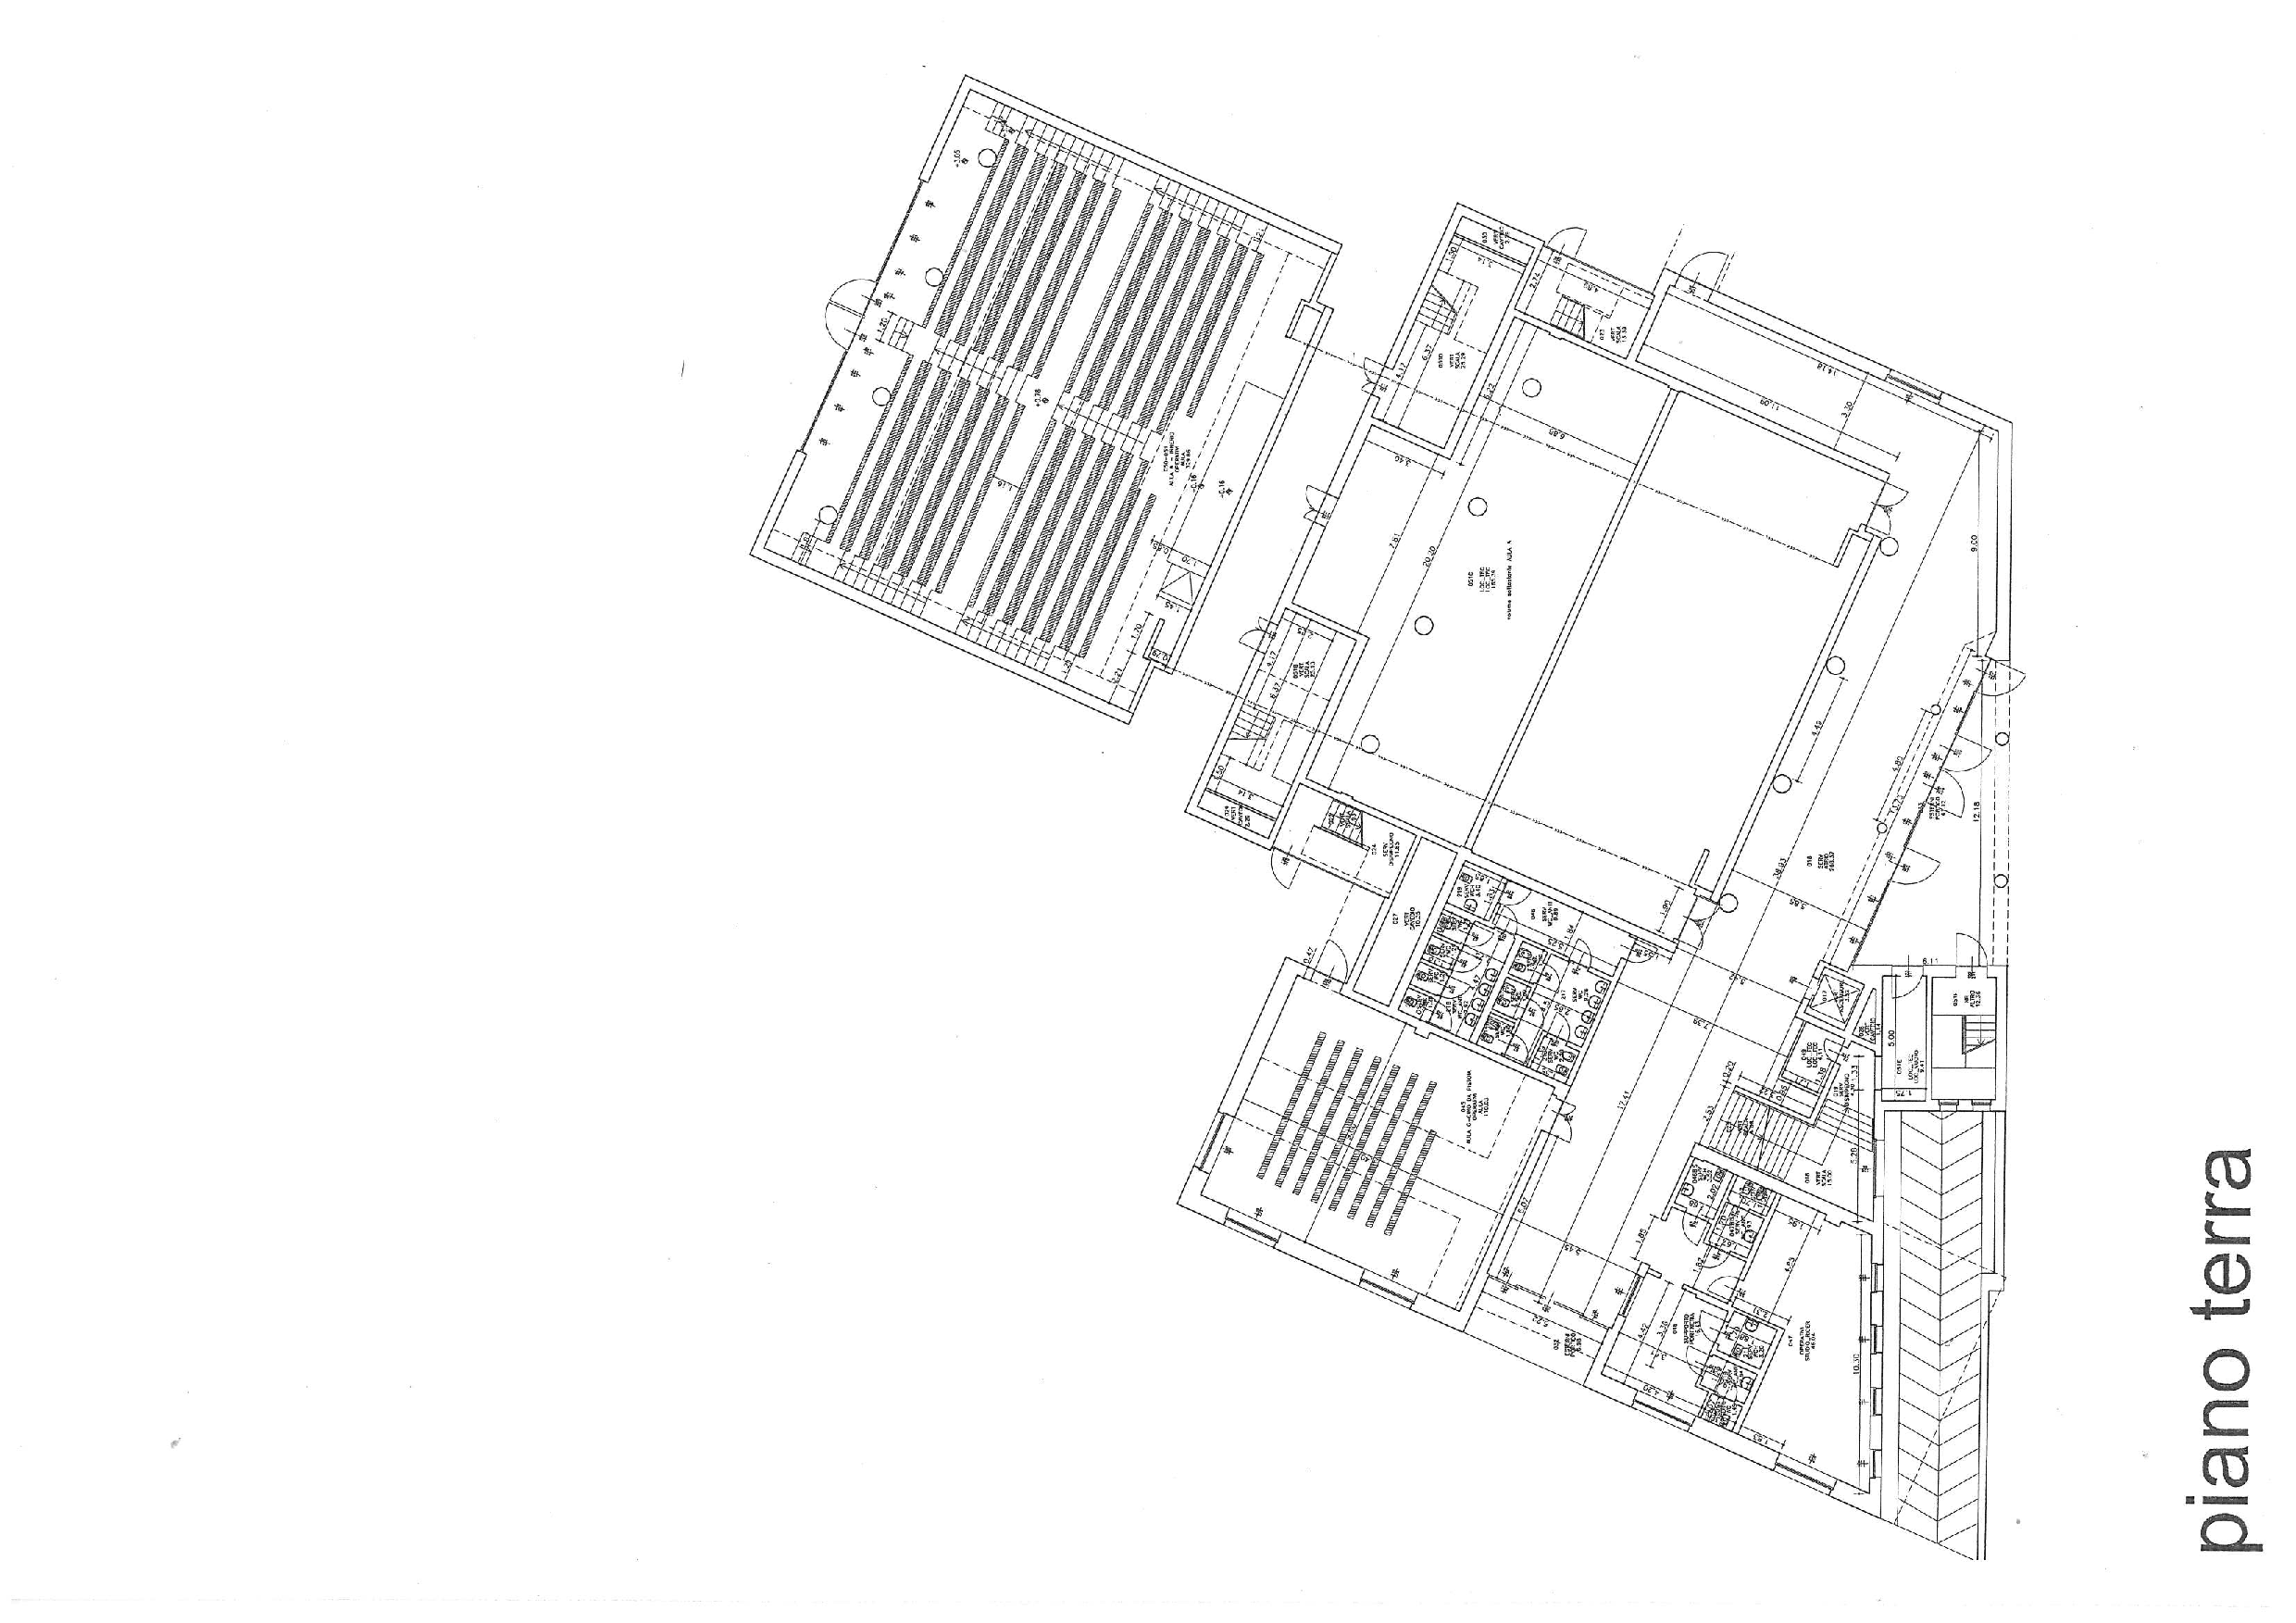
\includegraphics[scale=0.25]{A0.pdf}
\newpage
\begin{multicols}{2}
%-----Registration Desk
\section*{Registration Desk}
\addcontentsline{toc}{section}{Registration Desk}
The registration desk is located in the hall of Building A, via Belmeloro 14 and is open during the following hours:
\begin{itemize}
\item Monday, June 4: 3:30 PM - 6:30 PM
\item Tuesday, June 5: 12:00 PM - 6:30 PM
\item Wednesday, June 6: 8:30 AM - 6:30 PM
\item Thursday, June 7: 8:30 AM - 6:30 PM
\item Friday, June 8: 8:30 AM - 6:30 PM
\end{itemize}
%-----Name Badges
%-----Name Badges
\subsection*{Name Badges} Carry your badge during the conference so that you can be admitted to all technical sessions, coffee breaks, lunches, reception and banquet (2014)\\
A space for emergency contact information is provided on the back of your name badge. Help us, help you in the event of an emergency! (2016)
%-----Registration Fee Includes
\subsection*{Registration Fee Includes}
\begin{itemize}
\item Admission to all technical sessions
\item Business Meeting (open to SIAG/IS members)
\item Social Dinner
\item Coffee breaks daily
\item Welcome Lunch and Poster Session
\item Room set-ups and audio/visual equipment
\item Wi-Fi access at the conference
\end{itemize}%-----Conference Talk Arrangements
%-----Conference Talk Arrangements
\subsection*{Conference Talk Arrangements}
All plenary talks and SIAG prize lecture will be 45 minutes in duration,
with 5 of the 45 minutes reserved for questions and discussion.
%The Vicent Caselles student award
%talk will be 20 minutes in duration,
%with 5 of the 20 minutes reserved for
%questions and discussion.
The minitutorial will be 2 hours in duration.\\\\
All minisymposia talks will be 30 minutes in duration, with 5 of the 30
minutes reserved for questions and discussion.
All contributed talks will be 20 minutes in duration, with 5 of the 20
minutes reserved for questions and discussion.\\\\
In case you need to copy your presentation slides from your USB to a
computer in lecture hall or meeting room, please do it in advance before
the session starts.
%-----Important Notice to Poster Presenters
\subsection*{Important Notice to Poster Presenters}
The poster session is scheduled for
Tuesday, June 5 from 5:00 PM - 7:00 PM. Poster
presenters are requested to set up
their poster material on the provided
4'x6' (CONTROLLARE) poster boards at the WHERE between the hours of 12:00 AM and 5:00 PM. 
All materials must
be posted by ??? at
5:00 PM, the official start time of
the session. Posters will remain on display through WHEN.
Posters displays must be removed by this time. Posters remaining after this time will be discarded.
The conference is not responsible for
discarded posters.
%------------Wi-Fi Access
\section*{Wi-Fi Access}
The username and password of your account during the conference period (5-8 June) can be found.....
%-------------------Standard Audio/VIsual Set-Up in Meeting Rooms
\subsection*{Standard Audio/Visual Set-Up in Meeting Rooms}
The plenary session room has a PC, two screens and two data projectors.\\ 
All other concurrent/breakout rooms have a PC, a screen, a data projector and a whiteboard (overhead projectors are also available).\\
The data projectors support VGA connection only. Presenters requiring an HDMI or alternate connection must provide their own adaptor.\\
Cables or adaptors for Apple computers are not supplied, as they vary for each model: please bring your own cable/adaptor if using a Mac computer. 
The conference is not responsible for the safety and security of speakers' computers.\\
COME CI VOGLIAMO ORGANIZZARE???? Possono portare il loro computer? Vogliamo fare una cartella drive? 
%-------------Recording of presentations
\subsection*{Recording of Presentations}
Audio and video recording of presentations at the conference is prohibited without the written permission of the speaker and the conference.
%-------------SIAM Books and Journal
\subsection*{SIAM Books and Journals}CONTROLLARE
Display copies of books and complimentary copies of journals are available on site. SIAM books are available at a discounted price during the conference. The book booth will be staffed from 9:00 AM through 6:00 PM. \\If a SIAM books representative is temporarily away from the booth, completed order forms and payment (credit cards are preferred) may be taken to the registration desk. The books table will close at 4:00 PM on Friday??? (2016)\\
Completed order forms should be emailed or faxed to the SIAM office directly. It is not allowed to carry out on site transaction during the conference period??? (2014)
%------------------ GET TOGETHERS
\addcontentsline{toc}{section}{Get-togethers}
\subsection*{Get-togethers}
\begin{itemize}
\item Tuesday, June 5, 12:00 PM - 2:30 PM, Welcome Lunch
\item Tuesday, June 5, 5:00 PM - 7:00 PM, Poster Session I
\item Thursday, June 7, 5:00 PM - 7:00 PM, Poster Session II
\item Thursday, June 7, 6:00 PM - ....., SIAG/IS Business Meeting
\end{itemize}
%---------------Lunches
\subsection*{Lunches}
Dove andare a pranzo
%---------------Conference Banquet
\subsection*{Conference Banquet}
The Conference banquet will be served in.......\\ Additional conference banquet tickets are available: the price is 65 euros. Please check and buy at the registration desk before Tuesday, June 5 afternoon.
%---------------Child Care
\subsection*{Child Care}
bla bla bla bla bla bla bla bla bla bla bla bla bla bla bla bla bla bla bla bla bla bla bla bla bla bla bla bla bla bla bla bla
%---------------Please Note
\subsection*{Please note}
The conference is not responsible for the safety and security of participants' computers. Do not leave your laptop computers and personal thngs unattended. Please remember to turn off your cell phone, pagers, etc in all the sessions.\\\\ The conference cannot provide photocopying and dollar exchange service. The bank can be found in piazza Aldrovandi 12/A.
%---------------Comments
\subsection*{Comments?}
Comments about SIAM IS18 are encouraged! Please send it to Cynthia Phillips, SIAM Vice President for Programs (vpp@siam.org)
\end{multicols}
%----------------Conference Sponsors
\addcontentsline{toc}{section}{Sponsors and Exhibitors}
\section*{Conference Sponsors}

\includegraphics[scale=0.25]{images/logo_APT}

\includegraphics[scale=0.4]{images/logo_CINECA}\\

\includegraphics[scale=0.5]{images/logo_BPER}

\includegraphics[scale=0.4]{images/logo_TIPO}\\

\includegraphics[scale=0.5]{images/logo_SIMAI}

\includegraphics[scale=0.9]{images/logo_DATALOGIC}\\
%
\includegraphics[scale=0.9]{logo_AZIMUT}
%----------------Visit the exhibits!
\addcontentsline{toc}{section}{Visit the exhibits}
\section*{Visit the exhibits}
Exhibitors:
\begin{itemize}
\item ....
\item
\item ...
\end{itemize}



%----------------INVITED PLENARY PRESENTATIONS
{\small{Invited Plenary Presentations  IP1 and IP2 on Tuesday, June 5, will take place in Aula Santa Lucia, while the other Invited Presentation will take place in Building A, Rooms A and B in via Belmeloro 14}}
%\vspace{2cm}
%---IP1
\newpage\vspace{2cm}
\begin{center}{\Large{
Tuesday, June 5, 9:45 AM - 10:30 AM \\
\textbf{IP1: Linearly-convergent stochastic gradient algorithms}\\
Francis Bach, Departement d'Informatique de l'Ecole Normale Superieure Centre de Recherche INRIA de Paris, PARIS, France}}
\end{center}
\vspace{1cm}

\begin{wrapfloat}{figure}{o}{0pt}
\includegraphics[scale=1.25]{Francis_Bach.jpg}
\end{wrapfloat}

Francis Bach is a researcher at Inria, leading since 2011 the machine learning project-team, which is part of the Computer Science Department at Ecole Normale Sup\'erieure. He graduated from Ecole Polytechnique in 1997 and completed his Ph.D. in Computer Science at U.C. Berkeley in 2005, working with Professor Michael Jordan. He spent two years in the Mathematical Morphology group at Ecole des Mines de Paris, then he joined the computer vision project-team at Inria/Ecole Normale Sup\'erieure from 2007 to 2010. Francis Bach is primarily interested in machine learning, and especially in graphical models, sparse methods, kernel-based learning, large-scale convex optimization, computer vision and signal processing. He obtained in 2009 a Starting Grant and in 2016 a Consolidator Grant from the European Research Council, and received in 2012 the Inria young researcher prize. In 2015, he was program co-chair of the International Conference in Machine learning (ICML).\\\\

\textbf{Abstract:}\\

Many machine learning and signal processing problems are traditionally cast as convex optimization problems where the objective function is a sum of many simple terms. In this situation, batch algorithms compute gradients of the objective function by summing all individual gradients at every iteration and exhibit a linear convergence rate for strongly-convex problems. Stochastic methods rather select a single function at random at every iteration, classically leading to cheaper iterations but with a convergence rate which decays only as the inverse of the number of iterations. In this talk, I will present the stochastic averaged gradient (SAG) algorithm which is dedicated to minimizing finite sums of smooth functions; it has a linear convergence rate for strongly-convex problems, but with an iteration cost similar to stochastic gradient descent, thus leading to faster convergence for machine learning and signal processing problems. I will also mention several extensions, in particular to saddle-point problems, showing that this new class of incremental algorithms applies more generally.



%---IP2
\newpage\vspace{2cm}
\begin{center}{\Large{
Tuesday, June 5, 10:45 AM - 11:30 AM \\
\textbf{IP2: Flexible methodology for image segmentation}\\
Raymond H. Chan, Department of Mathematics, The Chinese University of Hong Kong,  Hong Kong}}
\end{center}
\vspace{1cm}

\begin{wrapfloat}{figure}{o}{0pt}
\includegraphics[scale=0.75]{Raymond_Chan.jpg}
\end{wrapfloat}

Raymond Chan obtained his PhD degree from The Courant Institute of Mathematical Sciences in 1985. He is now the Chairman of the Mathematics Department at The Chinese University of Hong Kong. He won a Leslie Fox Prize in 1989; a Feng Kang Prize in 1997; a Morningside Award in 1998; and 2011 Higher Education Outstanding Scientific Research Output Awards from the Ministry of Education in China. He was elected a SIAM Fellow in 2013. He has published 120 journal papers and has been in the ISI Science Citation List of Top 250 Highly-Cited Mathematicians in the world since 2004. Chan has served on the editorial boards of many journals, including: Journal of Mathematical Imaging and Vision, Journal of Scientific Computing, Numerical Linear Algebra with Applications, SIAM Journal on Imaging Sciences, and SIAM Journal on Scientific Computing. 

%---IP3
\newpage\vspace{2cm}
\begin{center}{\Large{
Wednesday, June 6, 8:30 AM - 9:15 AM \\
\textbf{IP3: Fast analog to digital compression for high resolution imaging}\\
Yonina Eldar, Department of EE Technion, Israel Institute of Technology, Haifa, Israel
}}\end{center}
\vspace{1cm}


\begin{wrapfloat}{figure}{o}{0pt}
\includegraphics[scale=0.05]{Yonina_Eldar_small2}
\end{wrapfloat}
Yonina C. Eldar is a Professor in the Department of Electrical Engineering at the Technion, Israel Institute of Technology, Haifa, where she holds the Edwards Chair in Engineering. 
She is also a Research Affiliate with the Research Laboratory of Electronics at MIT and a Visiting Professor at Duke University, and was a Visiting Professor at Stanford University. 
She received the B.Sc. degree in physics and the B.Sc. degree in electrical engineering both from Tel-Aviv University (TAU), Tel-Aviv, Israel, in 1995 and 1996, respectively, and the Ph.D. degree in electrical engineering and computer science from the Massachusetts Institute of Technology (MIT), Cambridge, in 2002.
She has received many awards for excellence in research and teaching, as
the IEEE Signal Processing Society Technical Achievement Award (2013), the IEEE/AESS Fred Nathanson Memorial Radar Award (2014) and the IEEE Kiyo Tomiyasu Award (2016).
She was a Horev Fellow of the Leaders in Science and Technology program at the Technion and an Alon Fellow. 
She received the Michael Bruno Memorial Award from the Rothschild Foundation, the Weizmann Prize for Exact Sciences, the Wolf Foundation Krill Prize for Excellence in Scientific Research, the Henry Taub Prize for Excellence in Research (twice), the Hershel Rich Innovation Award (three times), the Award for Women with Distinguished Contributions, the Andre and Bella Meyer Lectureship, the Career Development Chair at the Technion, the Muriel \& David Jacknow Award for Excellence in Teaching, and the Technion's Award for Excellence in Teaching (two times). 
She received several best paper awards and best demo awards together with her research students and colleagues and was selected as one of the 50 most influential women in Israel.
She is the Editor in Chief of Foundations and Trends in Signal Processing, a member of several IEEE Technical Committees and Award Committees, an IEEE Fellow, and a EURASIP Fellow.
She is also a member of the Young Israel Academy of Science and was a member of the Israel Committee for Higher Education.\\\\
\textbf{Abstract:}\\
The famous Shannon-Nyquist theorem has become a landmark in the development of digital signal processing. However, in many modern applications, the signal bandwidths have increased tremendously, while the acquisition capabilities have not scaled sufficiently fast. Consequently, conversion to digital has become a serious bottleneck. Furthermore, the resulting high rate digital data requires storage, communication and processing at very high rates which is computationally expensive and requires large amounts of power. In the context of medical imaging sampling at high rates often translates to high radiation dosages, increased scanning times, bulky medical devices, and limited resolution. In this talk, we present a framework for sampling and processing a wide class of wideband analog signals at rates far below Nyquist by exploiting signal structure and the processing task and show several demos of real-time sub-Nyquist prototypes. We then consider applications of these ideas to a variety of problems in medical and optical imaging including fast and quantitative MRI, wireless ultrasound, fast Doppler imaging, and correlation based super-resolution in microscopy and ultrasound which combines high spatial resolution with short integration time. We end by discussing several modern methods for structure-based phase retrieval which has applications in several areas of optical imaging.

%--IP4
\newpage\vspace{2cm}
\begin{center}{\Large{
Wednesday, June 6, 1:30 PM - 2:15 PM \\
\textbf{IP4: Fake ID documents and counterfeited products: overview of image analysis techniques to fight them}\\
Clarissa Mandridake, Surys Group, France}}
\end{center}
\vspace{1cm}

\begin{wrapfloat}{figure}{o}{0pt}
\includegraphics[scale=0.12]{Clarissa_Mandridake.jpg}
\end{wrapfloat}
Mrs Clarisse Manjary Mandridake received his PhD in Image and Signal Processing from the University of Bordeaux I, France, for her works on bi-dimensional signal decomposition applied to classification of textured images, done in Laboratoire Automatique Productique et Traitement du Signal, and in closed connection with ARIANA Project in INRIA Sophia-Antipolis. She joined the research team of Advestigo for her postdoc year in 2002. As a researcher at Advestigo and later at Hologram Industries (now renamed SURYS), she developed technologies for the representation, indexation and search of images and videos in large scale databases. She is now in charge of the coordination of the research project for the SURYS digital labs and animates the scientist partnerships with University labs. Her expertise covers Applied Mathematics, image characterization, fingerprinting and authentication on various physical supports, from ID documents to smartlabels. More recently, his area of interest is to contribute to technological innovation for use by poor countries or developing countries in order to help them put in place what is called "good governance". It is a sine qua non Condition for any future economic development.


%--IP5
\newpage\vspace{2cm}
\begin{center}{\Large{
Thursday, June 7, 1:30 PM - 2:15 PM \\
\textbf{IP5: The expanding role of inverse problems in informing climate science and policy}\\
Anna Michalak, Department of Global Ecology, Carnegie Institution for Science, Stanford, CA, USA}}
\end{center}
\vspace{1cm}

\begin{wrapfloat}{figure}{o}{0pt}
\includegraphics[scale=0.065]{Anna_Michalak_small}
\end{wrapfloat}
Dr. Anna M. Michalak is a faculty member in the Department of Global Ecology of the Carnegie Institution for Science in Stanford, California, and an Associate Professor in the Department of Earth System Science at Stanford University. Prior to joining Carnegie, she was the Frank and Brooke Transue Faculty Scholar and Associate Professor at the University of Michigan, Ann Arbor. Her research interests primarily lie in two areas. She explores the impacts of climate change and extreme events on freshwater and coastal water quality via influences on nutrient delivery to, and on conditions within, water bodies. She also studies the cycling and emissions of greenhouse gases at the Earth surface at regional to global scales ? scales directly relevant to informing climate science and policy ? primarily through the use of atmospheric observations that provide the clearest constraints at these critical scales. She is the recipient of numerous awards, including the Presidential Early Career Award for Scientists and Engineers (nominated by NASA), the NSF CAREER award, the Association of Environmental Engineering and Science Professors Outstanding Educator Award, and the Leopold Fellowship in environmental leadership. Dr. Michalak holds a B.Sc. from the University of Guelph, Canada, and M.S. and Ph.D. degrees from Stanford.

%--IP6
\newpage\vspace{2cm}
\begin{center}{\Large{
Friday, June 8, 1:30 PM - 2:15 PM \\
\textbf{IP6: Image Segmentation and Understanding: A Challenge for Mathematicians}\\
Christoph Schn\"{o}rr, Institute of Applied Mathematics, University of Heidelberg, Germany}}
\end{center}
\vspace{1cm}

\begin{wrapfloat}{figure}{o}{0pt}
\includegraphics[scale=0.25]{Schnoerr_small}
\end{wrapfloat}
Christoph Schn\"{o}rr received his degrees from the Technical University of Karlsruhe (today: Karlsruhe Institute of Technology) and the University of Hamburg, respectively. He worked as a researcher at the Fraunhofer Institut of Information and Data Processing in Karlsruhe before moving to the University of Hamburg. In 1998, he became full professor at the University of Mannheim, where he set up and directed the Computer Vision and Pattern Recognition Group. He moved to the Heidelberg University in 2008 where he is heading the Image and Pattern Analysis Group at the Institute of Applied Mathematics, which also is member of the Interdisciplinary Center for Scientific Computing.

Christoph Schn\"{o}rr has been coordinating 2010-2018 a research training group focusing on probabilistic graphical models and its applications to image analysis, funded by the German Science Foundation. He is one of 4 directors of the Heidelberg Collaboratory for Image Processing that implements and explores novel ways of combining basic strategic research in academia and research labs in industry, as part of the excellence initiative of the Heidelberg University. He served 2005-2014 as co-editor in chief of the International Journal of Computer Vision and currently as associate editor for the Journal of Mathematical Imaging and Vision and the SIAM Journal of Imaging Science.

His research interests include mathematical models of image analysis and numerical optimisation.




%-----------------PRIZE PRESENTATIONS 
\newpage
\section*{Prize Presentations}
\addcontentsline{toc}{section}{Prize Presentations}
{\small{All Prize Presentations will take place in Building A, Rooms A and B in via Belmeloro 14}}
\vspace{2cm}
\begin{center}
Thursday, June 7, 8:30 AM - 9:15 AM \\
\textbf{SP1} Prize\\
Title\\
who\\
\end{center}
\vspace{2cm}
\begin{center}
Friday, June 8, 8:30 AM - 9:15 AM \\
\textbf{SP2} Prize\\
Title\\
who\\
\end{center}



%--------------MINITUTORIALS
\newpage
\chapter*{Minitutorials and Biography}
\addcontentsline{toc}{section}{Minitutorials and Biography}

\begin{center}\textbf{Wednesday, June 6, \\9:30 AM - 11:30 AM \\Room B}\end{center}
\begin{center}
\textbf{MT1: Computational Uncertainty Quantification for Inverse Problems}\\
Organizer: John Bardsley, Department of Mathematical Sciences, The University of Montana, MT, USA
\end{center}

\vspace{1cm}
\begin{center}\textbf{Thursday, June 7, \\9:30 AM - 11:30 AM \\Room B}\end{center}
%\vspace{2cm}
\begin{center}
\textbf{MT2: Automated 3D reconstruction from satellite images}\\
Organizer: Gabriele Facciolo, Centre de math\'ematiques et de leurs applications [CMLA] - Ecole Normale Sup\'erieure de Cachan, France\\
with\\ Carlo de Franchis and Enric Meinhardt-Lopis - Ecole Normale Sup\'erieure de Cachan, France
\end{center}
\vspace{1cm}
\begin{center}\textbf{Friday, June 8, \\9:30 AM - 11:30 AM \\Room B}\end{center}
%\vspace{2cm}
\begin{center}
\textbf{MT3: Regularization of Inverse Problem}\\
Organizer: Otmar Scherzer, Computational Science Center, University of Vienna, Austria
\end{center}

\newpage
%---------MT1
\begin{center}\textbf{Wednesday, June 6, 9:30 AM - 11:30 AM, Room B}\end{center}
%\vspace{2cm}
\begin{center}
\textbf{MT1: Computational Uncertainty Quantification for Inverse Problems}\\
Organizer: John Bardsley, Department of Mathematical Sciences, The University of Montana, MT, USA
\end{center}
%\vspace{2cm}

\begin{wrapfloat}{figure}{o}{0pt}
\includegraphics[scale=0.98]{John_Bardsley.jpg}
\end{wrapfloat}
Dr. Johnathan M. Bardsley is Professor of Mathematics at the University of Montana (UM) in Missoula, Montana, USA. He received his PhD from Montana State University in 2002 under the direction of Professor Curtis R. Vogel, with a dissertation focused on computational inverse problems. He then spent one year as a post-doc at the Statistical and Applied Mathematical Sciences Institute, under the direction of Professor H. Thomas Banks. He began his current job at UM in 2003, and since then has spent two years abroad as a visiting Professor: first at the University of Helsinki in Finland in 2006-07; and then at the University of Otago in New Zealand in 2010-11. Dr. Bardsley has published over 45 refereed journal articles and has given many presentations on his research around the world. He also organized Montana Uncertainty Quantification, a conference/workshop that took place at UM in June 2015. Dr. Bardsley's current research is focused, broadly, on uncertainty quantification for inverse problems, and more specifically, on the development of Markov chain Monte Carlo methods for sampling from posterior distributions that arise in both linear and nonlinear inverse problems. He has a forthcoming book, titled Computational Methods and Uncertainty Quantification for Inverse Problems, that will be published by SIAM.\\

\textbf{Abstract:} 
The field of inverse problems is fertile ground for the development of computational uncertainty quantification methods. This is due to the fact that, on the one hand, inverse problems involve noisy measurements, leading naturally to statistical (and hence uncertainty) estimation problems. On the other hand, inverse problems involve physical models that, upon discretization, are known only up to a high-dimensional vector of parameters, making them computationally challenging. Estimating a high-dimensional parameter vector in a discretized physical model from measurements of model output defines computational inverse problems. Such problems are typically unstable in that the estimates don?t depend continuously on the measurements. Regularization is a technique that provides stability for inverse problems, and in the Bayesian setting, it is synonymous with the choice of the prior probability density function. Once a prior is chosen, the posterior probability density function results, and it is the solution of the inverse problem in the Bayesian setting. The posterior maximizer ? known as the MAP estimator ? provides a stable estimate of the unknown parameters. However, uncertainty quantification requires that we extract more information from the posterior, which often requires sampling. The posterior density functions that arise in typical inverse problems are high-dimensional, and are often non-Gaussian, making the corresponding sampling problems challenging. In this mini-tutorial, I will begin with a discussion of inverse problems, move on to Bayesian statistics and prior modeling using Markov random fields, and then end with a discussion of some Markov chain Monte Carlo methods for sampling from posterior density functions that arise in inverse problems. 


%----MT2
\vspace{2cm}
\begin{center}\textbf{Thursday, June 7, 9:30 AM - 11:30 AM, Room B}\end{center}
%\vspace{2cm}
\begin{center}
\textbf{MT2: Automated 3D reconstruction from satellite images}\\
Organizer: Gabriele Facciolo, Centre de math\'ematiques et de leurs applications [CMLA] - Ecole Normale Sup\'erieure de Cachan, France\\
with\\ Carlo de Franchis and Enric Meinhardt-Lopis - Ecole Normale Sup\'erieure de Cachan, France
\end{center}

%\vspace{2cm}
\begin{wrapfloat}{figure}{o}{0pt}
\includegraphics[scale=0.4]{gabriele_facciolo.jpg}
\end{wrapfloat}
Gabriele Facciolo received his B.Sc. and M.Sc. in computer science from Universidad de la Republica del Uruguay, and his Ph.D. (2011) from Universitat Pompeu Fabra under the supervision of Vicent Caselles. During his thesis he contributed to a pioneering mathematical formalization of the image inpainting problem, and a formulation of temporally consistent video editing robust to illumination changes. He joined Jean-Michel Morel's group at the \'{E}cole Normale Sup\'erieure Paris-Saclay in 2011 where he is currently associate research professor. He has participated in many industrial projects, creating image processing algorithms and transferring technology with the CNES, Schlumberger, DxO Labs, and the foundation BarcelonaMedia. He has more than ten years of experience designing algorithms for remote sensing applications and collaborating with the French Space Agency (CNES) as part of the MISS project (Mat\'ematiques de l'Imagerie St\'er\'eoscopique Spatiale). The 3D reconstruction algorithms and the satellite stereo pipeline (github.com/MISS3D/s2p) he and his team have created within the CMLA have been adopted as the CNES?s official stereo pipeline. He and his team also won the 2016 IARPA Multi-View Stereo 3D Mapping Challenge. He is one of the founding Editors of IPOL (www.ipol.im), the first journal publishing articles associated to online executable algorithms.\\

\textbf{Abstract:} 
Commercial spaceborne imaging is experiencing an unprecedented growth both in size of the constellations and resolution of the images. This is driven by applications ranging from geographic mapping to measuring glacier evolution, or rescue assistance for natural disasters. For all these applications it is critical to automatically extract and update elevation data from arbitrary collections of multi-date satellite images. This multi-date satellite stereo problem is a challenging application of 3D computer vision: images are taken at very different dates, from very different points of view, and under different lighting conditions. The case of urban scenes adds further difficulties because of occlusions and reflections.
This tutorial is a hands-on introduction to the manipulation of optical satellite images, using complete examples with python code. The objective is to provide all the tools needed to process and exploit the images for 3D reconstruction. We will present the essential modeling elements needed for building a stereo pipeline for satellite images. This includes the specifics of satellite imaging such as pushbroom sensor modeling, coordinate systems, and localization functions. Then we will review the main concepts and algorithms for stereovision and tailor them to the case of satellite images. Finally, we will bring together these elements to build a 3D reconstruction pipeline for multi-date satellite images.
%-----MT3
\newpage
\begin{center}\textbf{Friday, June 8, 9:30 AM - 11:30 AM, Room B}\end{center}
%\vspace{2cm}
\begin{center}
\textbf{MT3: Regularization of Inverse Problem}\\
Organizer: Otmar Scherzer, Computational Science Center, University of Vienna, Austria
\end{center}

%\vspace{2cm}
\begin{wrapfloat}{figure}{o}{0pt}
\includegraphics[scale=0.35]{otmar_scherzer.jpg}
\end{wrapfloat}
Otmar Scherzer received his PhD and Habilitation from the University of Linz (Austria) in 1990, 1995, respectively. He was a postdoc researcher at Texas A\&M University and the University of Delaware. He held professorships at the Ludwig Maximilian University Munich, University of Bayreuth, University of Innsbruck before he became professor at the University of Vienna, where he is now the head of the Computational Science Center. In addition he is research group leader of the ``Imaging and Inverse Problems Group'' of the Radon Institute of Computational and Applied Mathematics (RICAM) in Linz, which is an institute of the Austrian Academy of Sciences. Otmar Scherzer is an expert in regularization theory and mathematical imaging. He has about 200 publications in leading journals in these fields and is editor of about 10 journals and book series, including SIAM J. imaging Sciences. Moreover, he published two monographs, and edited several books, including the Handbook of Mathematical Imaging in three volumes. In 1991 he received the Theodor K\"orner Prize, the Prize of the Austrian Mathematical Society, the science prize of Tyrol, and in 1999 the START-prize of the Austrian Science Foundation, which is the highest award for young Austrian scientists in Austria. From 2010 to 2017 he has been Vice-president of the Inverse Problems International Association (IPIA).\\

\textbf{Abstract:} 
Inverse Problems is an interdisciplinary research area with profound applications in many areas of science, engineering, technology, and medicine.
Nowadays, a core technology for solving imaging problems are
regularization methods. The foundations of these approximation methods were laid by Tikhonov decades ago, when he generalized the classical definition of well-posedness. 
In the early days of regularization methods, they were analyzed
mostly theoretically, while later on numerics, efficient solutions, 
and applications of regularization methods became important.
This MT gives a survey on theoretical developments in regularization 
theory: Starting from quadratic regularization methods for linear ill-posed 
problems, to convex regularization, and to non-convex regularization methods 
of non-linear problems. 
The theoretical analysis will be supported by particular 
imaging examples.



%----------------PROGRAM SCHEDULE 1
%\newpage
%\section*{SIAM IS18 PROGRAM-1}
%\addcontentsline{toc}{section}{Program Schedule-1}
%\newpage
%\begin{multicols}{3}
%\noindent {\large\textbf{Monday 4 June}} \\\\
%\textbf{Registration}\\ 5:00 PM -8:00 PM\\
%where
%
%\columnbreak 
%\noindent {\large\textbf{Tuesday 5 June}} \\\\
%\textbf{Registration}\\ 8:00 AM -12:00 PM\\
%2:00 PM - 5:00 PM\\
%where\\\\
%\textbf{Conference Remarks}\\
%when\\
%where
%
%
%\columnbreak 
%\noindent {\large\textbf{Tuesday 5 June}} \\\\
%blablabla
%\end{multicols}
%

%----------------------------------------------------------------------------------------
%	PART II: PROGRAM
%----------------------------------------------------------------------------------------

\part{Program}


%%----------------PROGRAM SCHEDULE 2
%\newpage 
%\section*{SIAM IS18 PROGRAM-2}
%\addcontentsline{toc}{section}{Program Schedule-2}
%\newpage
%
%\begin{tabular}{|c|p{6.5cm}|l|}
%\hline
%\multicolumn{3}{|l|}{}\\
%\multicolumn{3}{|l|}{\textbf{\Large{Tuesday, 5th}}}\\
%\multicolumn{3}{|l|}{}\\\hline
%& &\\TIME & & ROOM\\& &\\\hline & &\\
%8:00 AM - 12:00 PM & Registration & Belmeloro1\\& &\\
%9:30 AM - 10:00 AM & Welcoming Remarks & Aula Absidale Santa Lucia \\& &\\
%10:00 AM - 10:45 AM & \bf{Plenary session IP1} & Aula Absidale Santa Lucia\\& \bf{Who:} a very long title&\\& &\\
%10:45 AM - 11:30 AM & \bf{Plenary session IP2} & Aula Absidale Santa Lucia\\& \bf{Who:} a very very long and interesting title&\\& &\\
%12:30 PM & Lunch & Belmeloro \\& &\\
%14:00 PM - 16:00 PM & MS session 1 &  \\& &\\
%16:00 PM - 16:30 PM & Coffee break &  \\& &\\
%16:30 PM - 18:30 PM & MS session 2 &  \\& &\\
%
%\hline
%\end{tabular}
%
%\newpage
%\begin{tabular}{|p{12.5cm}|l|}
%\hline
%\multicolumn{2}{|l|}{}\\
%\multicolumn{2}{|l|}{\textbf{\Large{Tuesday, 5th}}}\\
%\multicolumn{2}{|l|}{}\\\hline
% &\\ LIST OF MS SESSION 1  14:00 PM - 16:00 PM & ROOM\\ &\\\hline  &\\
% MS1 Inversion of Non-linear Image Formation Models (Part I of II)  & Belmeloro A \\
% Organizers: bla bla bla & \\ &\\
% 
%  MS2 Recent Advances in Convex Relaxations (Part I of II)  & Belmeloro B \\
% Organizers: bla bla bla & \\ &\\
% 
%  MS3 Recent Advances in Dictionary Learning (Part I of II)  & Belmeloro C \\
% Organizers: bla bla bla & \\ &\\
% 
%  MS4 Statistical Methods for Inverse Problems Involving Partial Differential Equations & Belmeloro D \\
% Organizers: bla bla bla & \\ &\\
% 
%  MS5 Multi-Modality Imagining and Structural Priors (Part I of II)  & Belmeloro E \\
% Organizers: bla bla bla & \\ &\\
% 
%  MS6 Image Segmentation, Classification and Application (Part I of II)  & Belmeloro F \\
% Organizers: bla bla bla & \\ &\\
% 
%  MS7 Computational Metods for Inverse Problems in Imagining  & Belmeloro G \\
% Organizers: bla bla bla & \\ &\\
% 
%  MS8 Non-Gaussian Noise: New Trends and Challenges (Part I of II)  & Belmeloro H \\
% Organizers: bla bla bla & \\ &\\
%  MS9 Efficient Algorithms for Large-scale Inverse Problems in Medical Imagining (Part I of II)  & Belmeloro I \\
% Organizers: bla bla bla & \\ &\\
%  MS10 Image Analysis Advances in Dynamic Microscopy and Live Cell Imaging (Part I of II)  & Belmeloro J \\
% Organizers: bla bla bla & \\ &\\
% \hline
%
% \end{tabular}
% 
% \begin{tabular}{|p{12.5cm}|l|}
%\hline
%\multicolumn{2}{|l|}{}\\
%\multicolumn{2}{|l|}{\textbf{\Large{Tuesday, 5th}}}\\
%\multicolumn{2}{|l|}{}\\\hline
% &\\ LIST OF MS SESSION 32  16:00 PM - 18:00 PM & ROOM\\ &\\\hline  &\\
% MS11 Inversion of Non-linear Image Formation Models (Part I of II)  & Belmeloro A \\
% Organizers: bla bla bla & \\ &\\
% 
%  MS12 Recent Advances in Convex Relaxations (Part I of II)  & Belmeloro B \\
% Organizers: bla bla bla & \\ &\\
% 
%  MS13 Recent Advances in Dictionary Learning (Part I of II)  & Belmeloro C \\
% Organizers: bla bla bla & \\ &\\
% 
%  MS14 Statistical Methods for Inverse Problems Involving Partial Differential Equations & Belmeloro D \\
% Organizers: bla bla bla & \\ &\\
% 
%  MS15 Multi-Modality Imagining and Structural Priors (Part I of II)  & Belmeloro E \\
% Organizers: bla bla bla & \\ &\\
% 
%  MS16 Image Segmentation, Classification and Application (Part I of II)  & Belmeloro F \\
% Organizers: bla bla bla & \\ &\\
% 
%  MS17 Computational Metods for Inverse Problems in Imagining  & Belmeloro G \\
% Organizers: bla bla bla & \\ &\\
% 
%  MS18 Non-Gaussian Noise: New Trends and Challenges (Part I of II)  & Belmeloro H \\
% Organizers: bla bla bla & \\ &\\
%  MS19 Efficient Algorithms for Large-scale Inverse Problems in Medical Imagining (Part I of II)  & Belmeloro I \\
% Organizers: bla bla bla & \\ &\\
%  MS20 Image Analysis Advances in Dynamic Microscopy and Live Cell Imaging (Part I of II)  & Belmeloro J \\
% Organizers: bla bla bla & \\ &\\
% \hline
%
% \end{tabular}


\include{minisyposia_abstracts.tex}
%----------------------------------------------------------------------------------------
%	PART III: Abstracts
%----------------------------------------------------------------------------------------

\part{Abstracts}


%%Abstracts of Minysimposia Talks

\chapter*{Abstracts of Minysimposia Talks}

\begin{multicols}{2}
\noindent\textbf{MS01 Part I}\\
\textbf{Title}\\
 This is an abstract. This is an abstract. This is an abstract. This is an abstract. This is an abstract. This is an abstract. This is an abstract. This is an abstract. This is an abstract. This is an abstract. This is an abstract. This is an abstract. This is an abstract. This is an abstract. This is an abstract. This is an abstract. This is an abstract. This is an abstract. This is an abstract. This is an abstract. This is an abstract. This is an abstract. This is an abstract. This is an abstract. This is an abstract. This is an abstract. \\It's not very interesting\\\\
\myaut{Author}\\
University of....\\
\mail{nothing@gmail.com}\\\\

\noindent\textbf{MS01 Part I}\\
\textbf{Title}\\
This is an abstract. This is an abstract. This is an abstract. This is an abstract. This is an abstract. This is an abstract. This is an abstract. This is an abstract. This is an abstract. This is an abstract. This is an abstract. This is an abstract. This is an abstract. This is an abstract. This is an abstract. This is an abstract. This is an abstract. This is an abstract. This is an abstract. This is an abstract. This is an abstract. This is an abstract. This is an abstract. This is an abstract. This is an abstract. This is an abstract. This is an abstract. This is an abstract. This is an abstract. This is an abstract. This is an abstract. This is an abstract. \\It's not very interesting\\\\
\myaut{Author}\\
University of....\\
\mail{nothing@gmail.com}\\\\

\noindent\textbf{MS01 Part I}\\
\textbf{Title}\\
This is an abstract. This is an abstract. This is an abstract. This is an abstract. This is an abstract. This is an abstract. This is an abstract. This is an abstract. This is an abstract. This is an abstract. This is an abstract. This is an abstract. This is an abstract. This is an abstract. This is an abstract. This is an abstract. This is an abstract. This is an abstract. This is an abstract. This is an abstract. This is an abstract. This is an abstract. This is an abstract. This is an abstract. This is an abstract. This is an abstract. This is an abstract. This is an abstract. This is an abstract. This is an abstract. This is an abstract. This is an abstract. \\It's not very interesting\\\\
\myaut{Author}\\
University of....\\
\mail{nothing@gmail.com}\\\\

\noindent\textbf{MS01 Part I}\\
\textbf{Title}\\
This is an abstract. This is an abstract. This is an abstract. This is an abstract. This is an abstract. This is an abstract. This is an abstract. This is an abstract. This is an abstract. This is an abstract. This is an abstract. This is an abstract. This is an abstract. This is an abstract. This is an abstract. This is an abstract. This is an abstract. This is an abstract. This is an abstract. This is an abstract. This is an abstract. This is an abstract. This is an abstract. This is an abstract. This is an abstract. This is an abstract. This is an abstract. This is an abstract. This is an abstract. This is an abstract. This is an abstract. This is an abstract. \\It's not very interesting\\\\
\myaut{Author}\\
University of....\\
\mail{nothing@gmail.com}\\\\

\noindent\textbf{MS01 Part II}\\
\textbf{Title}\\
This is an abstract. This is an abstract. This is an abstract. This is an abstract. This is an abstract. This is an abstract. This is an abstract. This is an abstract. This is an abstract. This is an abstract. This is an abstract. This is an abstract. This is an abstract. This is an abstract. This is an abstract. This is an abstract. This is an abstract. This is an abstract. This is an abstract. This is an abstract. This is an abstract. This is an abstract. This is an abstract. This is an abstract. This is an abstract. This is an abstract. This is an abstract. This is an abstract. This is an abstract. This is an abstract. This is an abstract. This is an abstract. \\It's not very interesting\\\\
\myaut{Francy}\\
University of....\\
\mail{nothing@gmail.com}\\\\

\end{multicols}


%----------------------------------------------------------------------------------------
%	PART III: Abstracts
%----------------------------------------------------------------------------------------

\part{Abstracts}


%%Abstracts of Minysimposia Talks

\chapter*{Abstracts of Minysimposia Talks}

\begin{multicols}{2}
\noindent\textbf{MS01 Part I}\\
\textbf{Title}\\
 This is an abstract. This is an abstract. This is an abstract. This is an abstract. This is an abstract. This is an abstract. This is an abstract. This is an abstract. This is an abstract. This is an abstract. This is an abstract. This is an abstract. This is an abstract. This is an abstract. This is an abstract. This is an abstract. This is an abstract. This is an abstract. This is an abstract. This is an abstract. This is an abstract. This is an abstract. This is an abstract. This is an abstract. This is an abstract. This is an abstract. \\It's not very interesting\\\\
\myaut{Author}\\
University of....\\
\mail{nothing@gmail.com}\\\\

\noindent\textbf{MS01 Part I}\\
\textbf{Title}\\
This is an abstract. This is an abstract. This is an abstract. This is an abstract. This is an abstract. This is an abstract. This is an abstract. This is an abstract. This is an abstract. This is an abstract. This is an abstract. This is an abstract. This is an abstract. This is an abstract. This is an abstract. This is an abstract. This is an abstract. This is an abstract. This is an abstract. This is an abstract. This is an abstract. This is an abstract. This is an abstract. This is an abstract. This is an abstract. This is an abstract. This is an abstract. This is an abstract. This is an abstract. This is an abstract. This is an abstract. This is an abstract. \\It's not very interesting\\\\
\myaut{Author}\\
University of....\\
\mail{nothing@gmail.com}\\\\

\noindent\textbf{MS01 Part I}\\
\textbf{Title}\\
This is an abstract. This is an abstract. This is an abstract. This is an abstract. This is an abstract. This is an abstract. This is an abstract. This is an abstract. This is an abstract. This is an abstract. This is an abstract. This is an abstract. This is an abstract. This is an abstract. This is an abstract. This is an abstract. This is an abstract. This is an abstract. This is an abstract. This is an abstract. This is an abstract. This is an abstract. This is an abstract. This is an abstract. This is an abstract. This is an abstract. This is an abstract. This is an abstract. This is an abstract. This is an abstract. This is an abstract. This is an abstract. \\It's not very interesting\\\\
\myaut{Author}\\
University of....\\
\mail{nothing@gmail.com}\\\\

\noindent\textbf{MS01 Part I}\\
\textbf{Title}\\
This is an abstract. This is an abstract. This is an abstract. This is an abstract. This is an abstract. This is an abstract. This is an abstract. This is an abstract. This is an abstract. This is an abstract. This is an abstract. This is an abstract. This is an abstract. This is an abstract. This is an abstract. This is an abstract. This is an abstract. This is an abstract. This is an abstract. This is an abstract. This is an abstract. This is an abstract. This is an abstract. This is an abstract. This is an abstract. This is an abstract. This is an abstract. This is an abstract. This is an abstract. This is an abstract. This is an abstract. This is an abstract. \\It's not very interesting\\\\
\myaut{Author}\\
University of....\\
\mail{nothing@gmail.com}\\\\

\noindent\textbf{MS01 Part II}\\
\textbf{Title}\\
This is an abstract. This is an abstract. This is an abstract. This is an abstract. This is an abstract. This is an abstract. This is an abstract. This is an abstract. This is an abstract. This is an abstract. This is an abstract. This is an abstract. This is an abstract. This is an abstract. This is an abstract. This is an abstract. This is an abstract. This is an abstract. This is an abstract. This is an abstract. This is an abstract. This is an abstract. This is an abstract. This is an abstract. This is an abstract. This is an abstract. This is an abstract. This is an abstract. This is an abstract. This is an abstract. This is an abstract. This is an abstract. \\It's not very interesting\\\\
\myaut{Francy}\\
University of....\\
\mail{nothing@gmail.com}\\\\

\end{multicols}


%----------------------------------------------------------------------------------------
%	PART III: Abstracts
%----------------------------------------------------------------------------------------

\part{Abstracts}


%%Abstracts of Minysimposia Talks

\chapter*{Abstracts of Minysimposia Talks}

\begin{multicols}{2}
\noindent\textbf{MS01 Part I}\\
\textbf{Title}\\
 This is an abstract. This is an abstract. This is an abstract. This is an abstract. This is an abstract. This is an abstract. This is an abstract. This is an abstract. This is an abstract. This is an abstract. This is an abstract. This is an abstract. This is an abstract. This is an abstract. This is an abstract. This is an abstract. This is an abstract. This is an abstract. This is an abstract. This is an abstract. This is an abstract. This is an abstract. This is an abstract. This is an abstract. This is an abstract. This is an abstract. \\It's not very interesting\\\\
\myaut{Author}\\
University of....\\
\mail{nothing@gmail.com}\\\\

\noindent\textbf{MS01 Part I}\\
\textbf{Title}\\
This is an abstract. This is an abstract. This is an abstract. This is an abstract. This is an abstract. This is an abstract. This is an abstract. This is an abstract. This is an abstract. This is an abstract. This is an abstract. This is an abstract. This is an abstract. This is an abstract. This is an abstract. This is an abstract. This is an abstract. This is an abstract. This is an abstract. This is an abstract. This is an abstract. This is an abstract. This is an abstract. This is an abstract. This is an abstract. This is an abstract. This is an abstract. This is an abstract. This is an abstract. This is an abstract. This is an abstract. This is an abstract. \\It's not very interesting\\\\
\myaut{Author}\\
University of....\\
\mail{nothing@gmail.com}\\\\

\noindent\textbf{MS01 Part I}\\
\textbf{Title}\\
This is an abstract. This is an abstract. This is an abstract. This is an abstract. This is an abstract. This is an abstract. This is an abstract. This is an abstract. This is an abstract. This is an abstract. This is an abstract. This is an abstract. This is an abstract. This is an abstract. This is an abstract. This is an abstract. This is an abstract. This is an abstract. This is an abstract. This is an abstract. This is an abstract. This is an abstract. This is an abstract. This is an abstract. This is an abstract. This is an abstract. This is an abstract. This is an abstract. This is an abstract. This is an abstract. This is an abstract. This is an abstract. \\It's not very interesting\\\\
\myaut{Author}\\
University of....\\
\mail{nothing@gmail.com}\\\\

\noindent\textbf{MS01 Part I}\\
\textbf{Title}\\
This is an abstract. This is an abstract. This is an abstract. This is an abstract. This is an abstract. This is an abstract. This is an abstract. This is an abstract. This is an abstract. This is an abstract. This is an abstract. This is an abstract. This is an abstract. This is an abstract. This is an abstract. This is an abstract. This is an abstract. This is an abstract. This is an abstract. This is an abstract. This is an abstract. This is an abstract. This is an abstract. This is an abstract. This is an abstract. This is an abstract. This is an abstract. This is an abstract. This is an abstract. This is an abstract. This is an abstract. This is an abstract. \\It's not very interesting\\\\
\myaut{Author}\\
University of....\\
\mail{nothing@gmail.com}\\\\

\noindent\textbf{MS01 Part II}\\
\textbf{Title}\\
This is an abstract. This is an abstract. This is an abstract. This is an abstract. This is an abstract. This is an abstract. This is an abstract. This is an abstract. This is an abstract. This is an abstract. This is an abstract. This is an abstract. This is an abstract. This is an abstract. This is an abstract. This is an abstract. This is an abstract. This is an abstract. This is an abstract. This is an abstract. This is an abstract. This is an abstract. This is an abstract. This is an abstract. This is an abstract. This is an abstract. This is an abstract. This is an abstract. This is an abstract. This is an abstract. This is an abstract. This is an abstract. \\It's not very interesting\\\\
\myaut{Francy}\\
University of....\\
\mail{nothing@gmail.com}\\\\

\end{multicols}


%%--------------------- Abstracts of Contributed talks
\chapter*{Abstracts of  Contributed Talks}

\begin{multicols}{2}
\noindent\textbf{CT01}\\
\textbf{Title}\\
This is an abstract. This is an abstract. This is an abstract. This is an abstract. This is an abstract. This is an abstract. This is an abstract. This is an abstract. This is an abstract. This is an abstract. This is an abstract. This is an abstract. This is an abstract. This is an abstract. This is an abstract. This is an abstract. This is an abstract. This is an abstract. This is an abstract. This is an abstract. This is an abstract. This is an abstract. This is an abstract. This is an abstract. This is an abstract. This is an abstract. This is an abstract. This is an abstract. This is an abstract. This is an abstract. This is an abstract. This is an abstract. \\It's not very interesting\\\\
\myaut{Author}\\
University of....\\
\mail{nothing@gmail.com}\\\\

\noindent\textbf{CT02}\\
\textbf{Title}\\
This is an abstract. This is an abstract. This is an abstract. This is an abstract. This is an abstract. This is an abstract. This is an abstract. This is an abstract. This is an abstract. This is an abstract. This is an abstract. This is an abstract. This is an abstract. This is an abstract. This is an abstract. This is an abstract. This is an abstract. This is an abstract. This is an abstract. This is an abstract. This is an abstract. This is an abstract. This is an abstract. This is an abstract. This is an abstract. This is an abstract. This is an abstract. This is an abstract. This is an abstract. This is an abstract. This is an abstract. This is an abstract. \\It's not very interesting\\\\
\myaut{Author}\\
University of....\\
\mail{nothing@gmail.com}\\\\

\noindent\textbf{CT03}\\
\textbf{Title}\\
This is an abstract. This is an abstract. This is an abstract. This is an abstract. This is an abstract. This is an abstract. This is an abstract. This is an abstract. This is an abstract. This is an abstract. This is an abstract. This is an abstract. This is an abstract. This is an abstract. This is an abstract. This is an abstract. This is an abstract. This is an abstract. This is an abstract. This is an abstract. This is an abstract. This is an abstract. This is an abstract. This is an abstract. This is an abstract. This is an abstract. This is an abstract. This is an abstract. This is an abstract. This is an abstract. This is an abstract. This is an abstract. \\It's not very interesting\\\\
\myaut{Author}\\
University of....\\
\mail{nothing@gmail.com}\\\\
\end{multicols}



\newpage
\thispagestyle{empty}
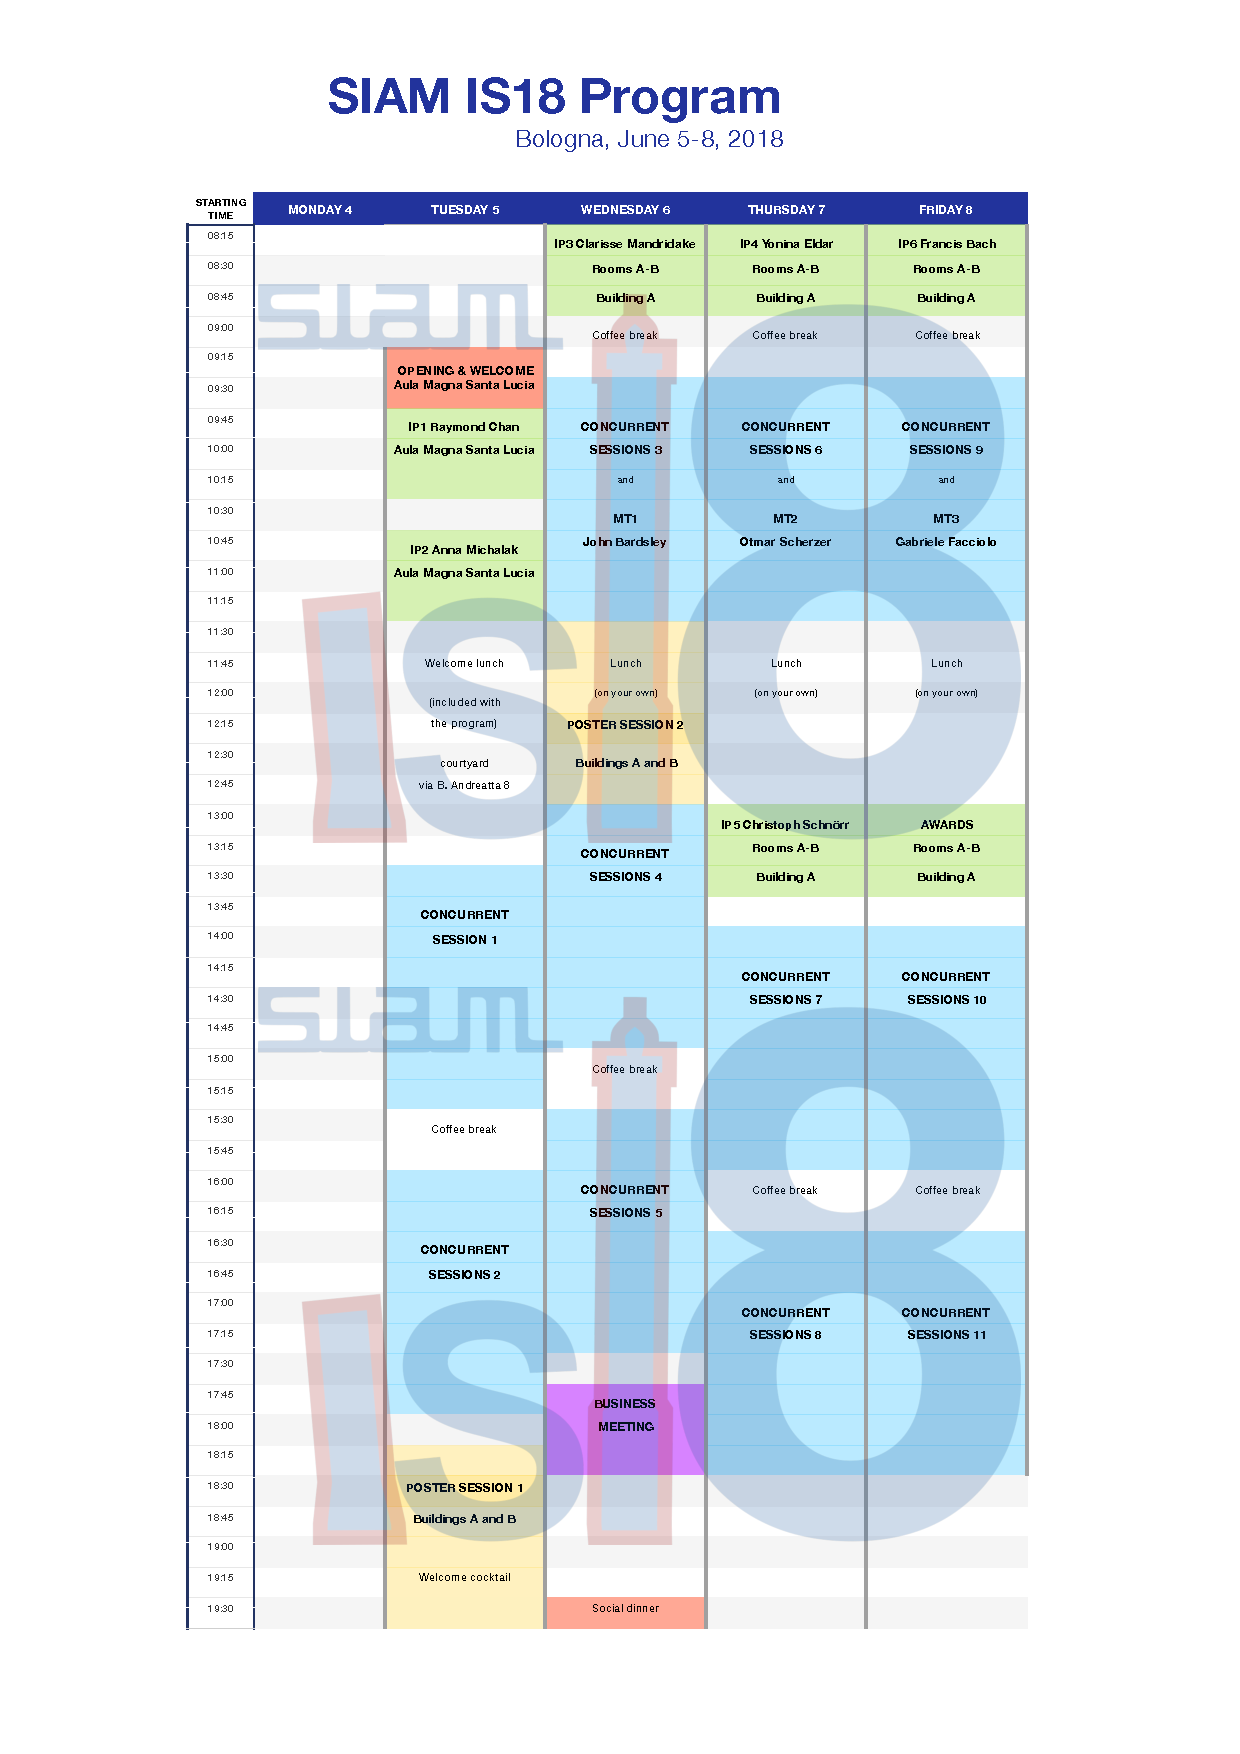
\includegraphics[scale=0.6]{program_table.pdf}
%
%
\end{document}
